% Options for packages loaded elsewhere
\PassOptionsToPackage{unicode}{hyperref}
\PassOptionsToPackage{hyphens}{url}
%
\documentclass[
]{book}
\usepackage{amsmath,amssymb}
\usepackage{lmodern}
\usepackage{ifxetex,ifluatex}
\ifnum 0\ifxetex 1\fi\ifluatex 1\fi=0 % if pdftex
  \usepackage[T1]{fontenc}
  \usepackage[utf8]{inputenc}
  \usepackage{textcomp} % provide euro and other symbols
\else % if luatex or xetex
  \usepackage{unicode-math}
  \defaultfontfeatures{Scale=MatchLowercase}
  \defaultfontfeatures[\rmfamily]{Ligatures=TeX,Scale=1}
\fi
% Use upquote if available, for straight quotes in verbatim environments
\IfFileExists{upquote.sty}{\usepackage{upquote}}{}
\IfFileExists{microtype.sty}{% use microtype if available
  \usepackage[]{microtype}
  \UseMicrotypeSet[protrusion]{basicmath} % disable protrusion for tt fonts
}{}
\makeatletter
\@ifundefined{KOMAClassName}{% if non-KOMA class
  \IfFileExists{parskip.sty}{%
    \usepackage{parskip}
  }{% else
    \setlength{\parindent}{0pt}
    \setlength{\parskip}{6pt plus 2pt minus 1pt}}
}{% if KOMA class
  \KOMAoptions{parskip=half}}
\makeatother
\usepackage{xcolor}
\IfFileExists{xurl.sty}{\usepackage{xurl}}{} % add URL line breaks if available
\IfFileExists{bookmark.sty}{\usepackage{bookmark}}{\usepackage{hyperref}}
\hypersetup{
  pdftitle={SQL Tutorial},
  pdfauthor={Autor: Jonathan Schuster},
  hidelinks,
  pdfcreator={LaTeX via pandoc}}
\urlstyle{same} % disable monospaced font for URLs
\usepackage{longtable,booktabs,array}
\usepackage{calc} % for calculating minipage widths
% Correct order of tables after \paragraph or \subparagraph
\usepackage{etoolbox}
\makeatletter
\patchcmd\longtable{\par}{\if@noskipsec\mbox{}\fi\par}{}{}
\makeatother
% Allow footnotes in longtable head/foot
\IfFileExists{footnotehyper.sty}{\usepackage{footnotehyper}}{\usepackage{footnote}}
\makesavenoteenv{longtable}
\usepackage{graphicx}
\makeatletter
\def\maxwidth{\ifdim\Gin@nat@width>\linewidth\linewidth\else\Gin@nat@width\fi}
\def\maxheight{\ifdim\Gin@nat@height>\textheight\textheight\else\Gin@nat@height\fi}
\makeatother
% Scale images if necessary, so that they will not overflow the page
% margins by default, and it is still possible to overwrite the defaults
% using explicit options in \includegraphics[width, height, ...]{}
\setkeys{Gin}{width=\maxwidth,height=\maxheight,keepaspectratio}
% Set default figure placement to htbp
\makeatletter
\def\fps@figure{htbp}
\makeatother
\setlength{\emergencystretch}{3em} % prevent overfull lines
\providecommand{\tightlist}{%
  \setlength{\itemsep}{0pt}\setlength{\parskip}{0pt}}
\setcounter{secnumdepth}{5}
\usepackage{booktabs}
\ifluatex
  \usepackage{selnolig}  % disable illegal ligatures
\fi
\usepackage[]{natbib}
\bibliographystyle{plainnat}

\title{SQL Tutorial}
\author{Autor: Jonathan Schuster}
\date{2021-11-10}

\begin{document}
\maketitle

{
\setcounter{tocdepth}{1}
\tableofcontents
}
\hypertarget{vorwort}{%
\chapter*{Vorwort}\label{vorwort}}
\addcontentsline{toc}{chapter}{Vorwort}

SQL (``Structured Query Language'') ist eine der meist genutzten Datenbanksprachen für relationale Datenbanken und findet sich in den unterschiedlichsten Branchen und Anwendungen wieder. Der Begriff relationale Datenbank beschreibt dabei eine Sammlung von Tabellen, die in Datensätzen abgespeichert werden und verknüpft werden können.

In diesem Tutorial werden die grundlegenden SQL Befehle und Funktionen anhand einer fiktiven Datenbank erklärt. Um den Einstieg so einfach wie möglich zu machen, wird dabei der \href{https://sqlitebrowser.org/}{DB Browser for SQLite verwendet}.

Weitere hilfreiche Ressourcen für den Einstieg lassen sich hier finden:

\hypertarget{setup}{%
\chapter{Setup}\label{setup}}

Im Folgenden werden wir uns zunächst einen Browser für \textbf{SQLite} und einen fiktiven Datensatz herunterladen. SQLite ist ein auf der Programmiersprache C beruhendes Datenbankmanagementsystem, das \textbf{ohne Serveranbindung} auf unserem Endsystem verwendet werden kann und uns daher ein wenig Aufwand erspart.

Bei vielen anderen Anwendungsfällen von SQL werden jedoch Datenbanksysteme genutzt, die auf Server zurückgreifen und daher erst eine speziellere Konfiguration benötigen. Da mittlerweile viele verschiedene Unternehmen oder Open Source Communities solche Datenbanksysteme auf Basis von \textbf{SQL Standards} entwickelt haben, gibt es leichte Unterschiede in einzelnen Syntax-Befehlen. Die zugrunde liegende Logik und die Funktionen sind jedoch deckungsgleich, sodass man mit Kenntnissen in einem Datenbanksystem problemlos auf andere SQL-Systeme umsteigen kann.

Die am stärksten verbreiteten Datenbanksysteme umfassen:

\begin{itemize}
\tightlist
\item
  MySQL - Open Source von Oracle\\
\item
  SQL Server - von Microsoft\\
\item
  PostgreSQL - Open Source\\
\item
  Oracle Database - von Oracle
\end{itemize}

\hypertarget{db-browser-for-sqlite-installation}{%
\section{DB Browser for SQLite Installation}\label{db-browser-for-sqlite-installation}}

Für einen einfachen Einstieg nutzen wir den kostenlosen \href{https://sqlitebrowser.org/}{DB Browser for SQLite}, der uns ohne großen Aufwand ermöglicht Datenbanken zu durchsuchen, Daten zu erstellen, Einträge zu bearbeiten, SQL Abfragen durchzuführen und Ergebnisse zu exportieren.

Der kostenfreie Download für Windows, macOS und Linux befindet sich hier:

\begin{itemize}
\tightlist
\item
  \href{https://sqlitebrowser.org/dl/}{DB Browser for SQLite Download}
\end{itemize}

Anschließend muss der Browser installiert werden.

\hypertarget{stunes-database}{%
\section{sTunes Database}\label{stunes-database}}

Als praktisches Beispiel für diese Einführung dient uns die Datenbank eines fiktiven Onlinestores für Musik. Wir simulieren also ein Szenario, in dem wir als Analysten für dieses fiktive Unternehmen tätig sind und im Auftrag unserer Stakeholder (Management, Investoren, Kunden, \ldots) beispielsweise Daten zu Alben, Artists, Kunden, Mitarbeitern, Genres, Umsätzen oder Bestelldetails sammeln und aufbereiten müssen. Wie genau diese Datenbank aufgebaut ist, werden wir uns noch anschauen.

Zunächst können wir die Datenbank unter folgendem Link mit dem Passwort ``IJK-Hannover''herunterladen:

\begin{itemize}
\tightlist
\item
  \href{https://1drv.ms/u/s!AqqMotwB6q520GDacSPl7I49CXPf?e=9ImRO2}{sTunes Datenbank Download}
\end{itemize}

Die zip-Datei können wir nun entpacken und die Datenbank-Datei in einem neuen Ordner abspeichern, in dem wir im folgenden auch unser Projekt anlegen.

\hypertarget{uxf6ffnen-der-datenbank}{%
\section{Öffnen der Datenbank}\label{uxf6ffnen-der-datenbank}}

Jetzt können wir den \textbf{DB Browser for SQLite} öffnen und uns mit dem Programm vertraut machen. Um unsere sTunes Datenbank zu öffnen, können wir auf \textbf{Datenbank öffnen} klicken und unsere \textbf{sTunes.db} Datei auswählen.

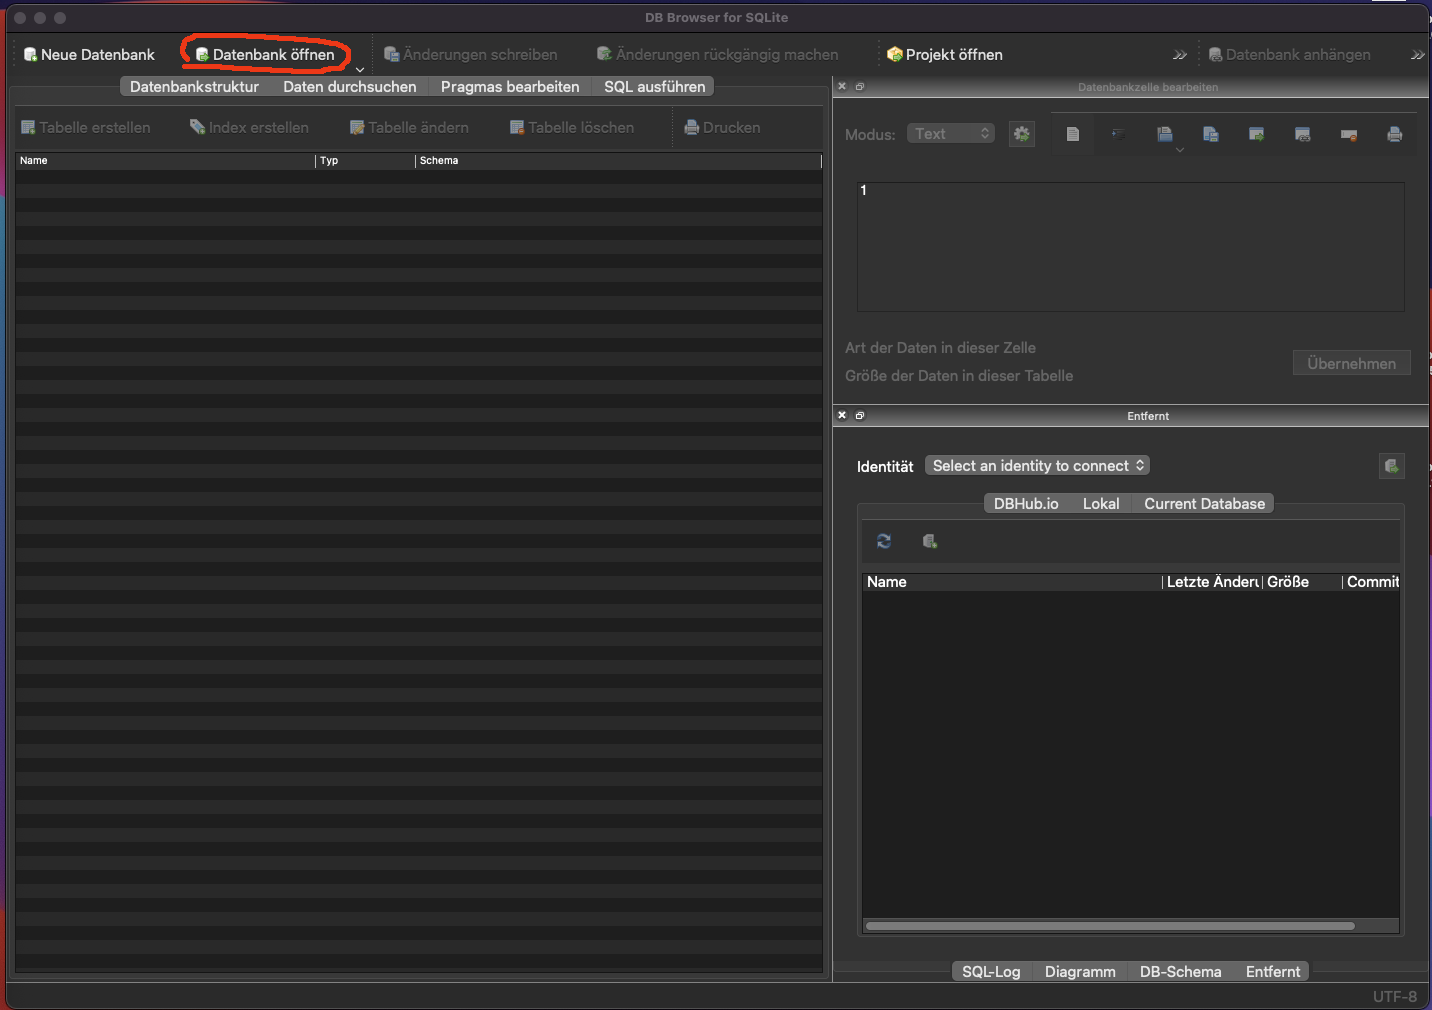
\includegraphics[width=\textwidth,height=5.20833in]{img-SQL-DBBrowser1.png}

\hypertarget{datenbank-schema}{%
\chapter{Datenbank Schema}\label{datenbank-schema}}

Nun sehen wir unter dem Reiter \textbf{Datenbankstruktur} welche Tabellen und dementsprechend welche Daten unsere Datenbank erhält. Wir sehen, dass die Datenbank \textbf{13 Tabellen} enthält und können uns für jede Tabelle anschauen, welche Variable unter welchem Namen gespeichert sind. So enthält unsere Tabelle \textbf{albums} die Variablen \textbf{AlbumID}, \textbf{Title} und \textbf{ArtistID}.

Die Spalte \emph{Typ} zeigt uns an, welches Format die Daten in der jeweiligen Tabellenspalte besitzen. Die Spalte \emph{Schema} zeigt uns, über welche Befehle die jeweiligen Tabellen und Spalten erstellt worden sind.

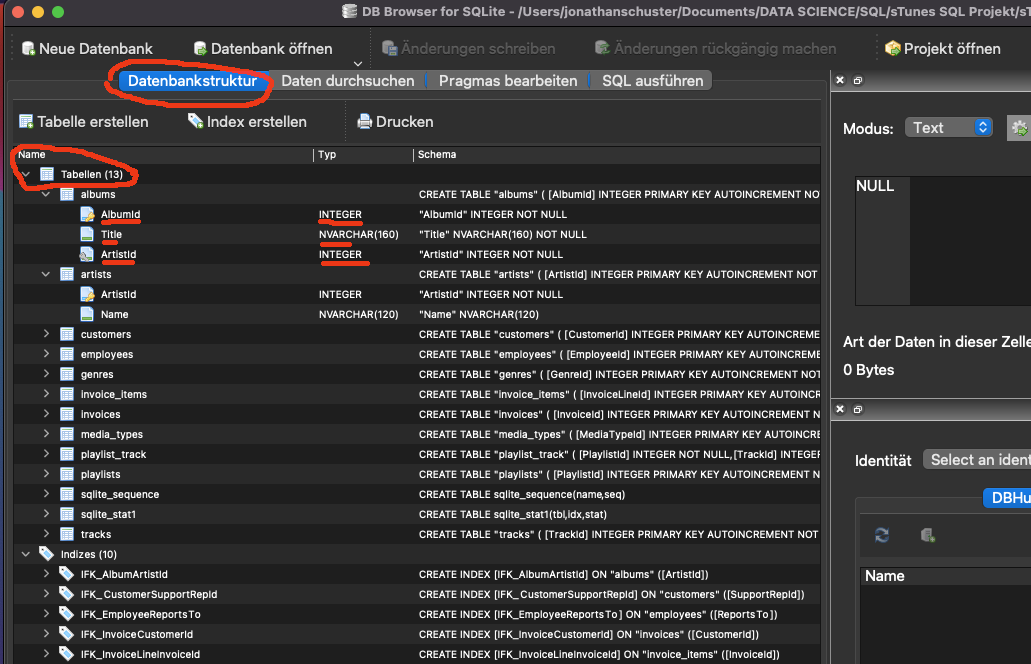
\includegraphics[width=\textwidth,height=5.20833in]{img-SQL-DBBrowser2.png}

Wir haben folglich also eine Übersicht zu allen Tabellen und ihren Variablen und können zum Beispiel folgende Rückschlüsse ziehen:

\begin{itemize}
\tightlist
\item
  Die Variable \textbf{AlbumID} in der Tabelle \textbf{albums} ist vom Typ \textbf{INTEGER}, also eine ganze Zahl.\\
\item
  Die Variable \textbf{Title} in der Tabelle \textbf{albums} ist vom Typ \textbf{NVARCHAR}, also eine Zeichenfolge mit variabler Länge und durch die Angabe \textbf{(160)} auf Maximal 160 Zeichen begrenzt.\\
\item
  Die Variable \textbf{UnitPrice} in der Tabelle \textbf{invoice\_items} ist vom Typ \textbf{NUMERIC}, also eine Zahl und durch die Angabe \textbf{(10,2)} auf insgesamt 10 Stellen begrenzt, wobei 2 dieser Stellen Nachkommastellen sind.
\end{itemize}

Eine Übersicht zu weiteren Datentypen ist hier zu finden:\\
\href{https://www.tutorialspoint.com/sqlite/sqlite_data_types.htm}{SQL Datatypes}

\hypertarget{entity-relationship-modell}{%
\section{Entity-Relationship-Modell}\label{entity-relationship-modell}}

Um das Schema der Datenbankstruktur zu veranschaulichen, habe ich die Tabellen mit ihren Variablen und den Beziehungen als sogenanntes \emph{Entity-Relationship-Modell}, kurz \emph{ERM} dargestellt. Dieses Modell hilft uns dabei, die Beziehungen der einzelnen Tabellen und ihrer Variablen zu veranschaulichen. Die Grafik ist zudem in unserem zip-Ordner zu finden:

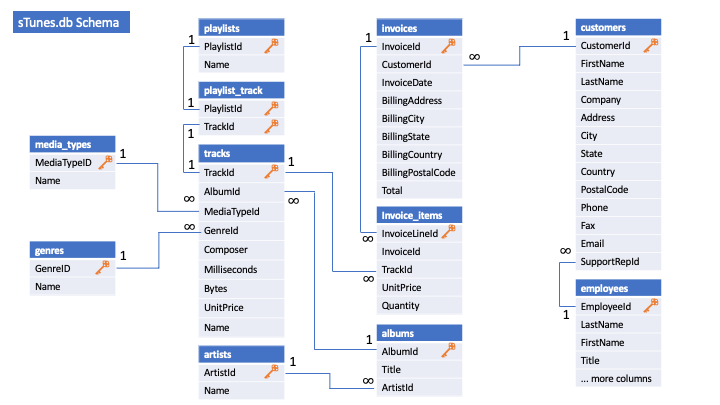
\includegraphics[width=10.41667in,height=\textheight]{img-sTunes-Schema.png}

Wir sehen hier, welche Tabellen in unserer Datenbank vorhanden sind, welche Variablen diese besitzen und wie diese Tabellen zueinander in Beziehung stehen.

\hypertarget{primary-foreign-keys}{%
\section{Primary \& Foreign Keys}\label{primary-foreign-keys}}

Zudem stellen wir fest, dass einige Variablen - in jeder Tabelle mindestens eine - mit einem Schlüsselsymbol versehen sind. Dieses Symbol zeigt uns, dass diese Variablen der sogenannte \textbf{PRIMARY KEY} in der jeweiligen Tabelle sind und als eindeutige Kennung (unique identifier) für die einzelnen Einträge in der Tabelle gelten.

So wissen wir beispielsweise, dass jedes einzelne Album in der Tabelle \textbf{albums}, also jeder einzelne Eintrag, eine eindeutige \textbf{AlbumId} besitzt über die das jeweilige Album identifiziert werden kann. Welche Variable als \textbf{PRIMARY KEY} dient, wird bei der Erstellung einer jeden Tabelle festgelegt. Ohne die Grafik würden wir die Info zu den Keys in unserer Übersicht zur Datenbankstruktur in der Spalte \emph{Schema} durch Hinweise wie \emph{{[}AlbumId{]} INTEGER PRIMARY KEY} finden. Wie wir anhand der Tabelle \textbf{playlist\_track} feststellen können, ist es auch möglich mehrere \textbf{PRIMARY KEYS} in einer Tabelle zu nutzen.

Folgen wir den Verbindungen der Variablen mit Schlüssel, den \textbf{PRIMARY KEYS} sehen wir, dass diese auch mit Variablen anderer Tabellen in Beziehung stehen, sogenannten \textbf{FOREIGN KEYS}. Ein \textbf{FOREIGN KEY} einer Tabelle ist eine Variable, die in einer anderen Tabelle als \textbf{PRIMARY KEY} verwendet wird. Diese Zuteilung ermöglicht es uns, die Daten aus verschiedenen Tabellen miteinander zu verbinden und auszuwerten.

Wir sehen beispielsweise, dass der PRIMARY KEY \textbf{ArtistID} in der Tabelle \textbf{artists} als FOREIGN KEY mit dem selben Namen in der Tabelle \textbf{albums} vorkommt. Nur durch diese Verknüpfung ist es beispielsweise möglich, den Namen aus der \textbf{artists} Tabelle an die Daten der \textbf{albums} Tabelle zu hängen, um eine Übersicht zu allen Alben und ihren Künstlern zu erstellen.

Die \textbf{Zahl 1} und das \textbf{Unendlichkeitszeichen} an den Verbindungen der Keys weisen zudem auf die Art der Beziehung hin. Während jeder Artist in der \textbf{artists} Tabelle nur einmal vorkommt und eine eindeutige \textbf{ArtistId} erhält, um Dopplungen zu vermeiden, kann diese \textbf{ArtistId} logischerweise bei unendlich vielen Alben vorkommen. Hat eine Künstlerin vier Alben gemacht, werden in der \textbf{albums} Tabelle vier Einträge mit eindeutigen \textbf{AlbumIds} vorkommen, die jedoch alle die selbe \textbf{ArtistId} verwenden.

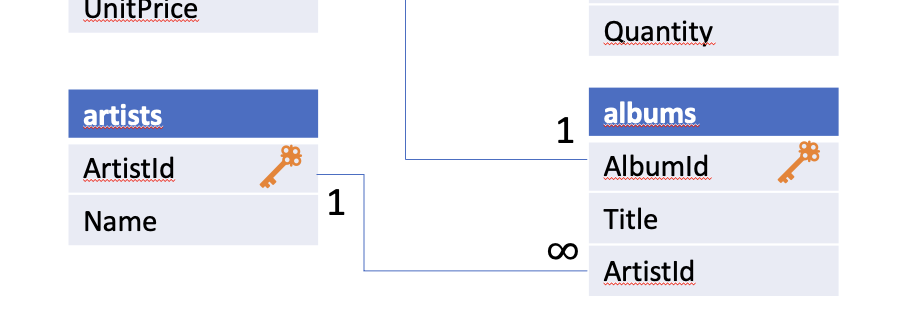
\includegraphics[width=10.41667in,height=\textheight]{img-sTunes-Schema2.png}

Zu beachten ist außerdem, dass ein PRIMARY KEY in einer Tabelle auch mit einem FOREIGN KEY mit anderem Namen in einer anderen Tabelle verbunden sein kann. So tritt der PRIMARY KEY \textbf{EmployeeId} der \textbf{employees} Tabelle als FOREIGN KEY mit dem Namen \textbf{SupportRepId} in der \textbf{customers} Tabelle auf. Während wir in der Personaltabelle vielleicht von Personalnummer sprechen, kann die gleiche Nummer in der Kundentabelle beispielsweise als Nummer der Betreuungsperson betitelt werden.

\hypertarget{sql-abfragen}{%
\chapter{SQL-Abfragen}\label{sql-abfragen}}

Nachdem wir uns einen Überblick über die Datenbankstruktur verschafft haben, können wir damit anfangen, Informationen aus unserer Datenbank abzufragen. Dazu müssen wir in unserem DB auf den Reiter \textbf{SQL ausführen} wechseln und können dann unsere Befehle in das Fenster schreiben. Durch den Play-Button lassen sich diese dann ausführen.

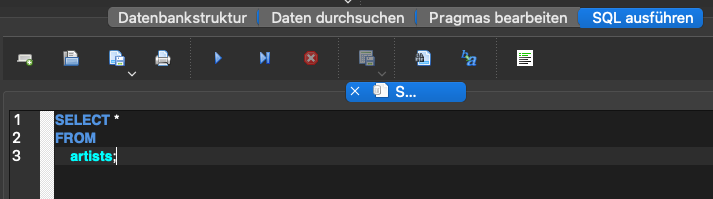
\includegraphics[width=10.41667in,height=\textheight]{img-SELECT1.png}

\hypertarget{select}{%
\section{SELECT}\label{select}}

Um Daten abzufragen, können wir das sogenannte \textbf{SELECT Statement} verwenden. Durch den folgenden Befehl können wir alle Einträge mit allen Spalten aus der Tabelle \textbf{artists} ausgeben lassen.

\begin{verbatim}
SELECT*
FROM
  artists;
\end{verbatim}

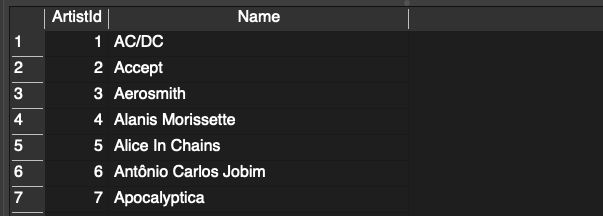
\includegraphics[width=10.41667in,height=\textheight]{img-SELECT2.png}

Durch das Sternchen haben wir alle Variablen ausgewählt. Möchten wir genauer festlegen, welche Variablen wir abfragen möchten, können wir dies zwischen \textbf{SELECT} und \textbf{FROM} definieren:

\begin{verbatim}
SELECT
  Name
FROM
  artists;
\end{verbatim}

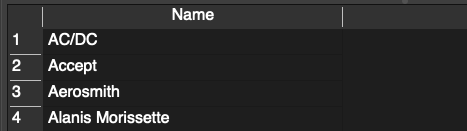
\includegraphics[width=10.41667in,height=\textheight]{img-SELECT3.png}

Dabei können wir beliebig viele Variablen wählen, indem wir sie durch ein Komma trennen. Nur bei der letzten Variable darf kein Komma stehen:

\begin{verbatim}
SELECT
  FirstName,
  LastName,
  Email
FROM
  customers;
\end{verbatim}

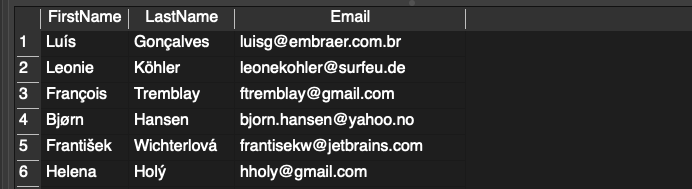
\includegraphics[width=10.41667in,height=\textheight]{img-SELECT4.png}

Um die Namen der Spalten in unserer Ausgabe zu verändern, können wir den ausgewählten Variablen in unserem SELECT Statement neu betiteln. Dabei reicht es bei einzelnen Worten den neuen Titel hinter die Zuordnung \textbf{AS} zu schreiben, während mehrere getrennte Worte wie im folgenden Beispiel durch '\,' oder {[} {]} umschlossen werden müssen:

\begin{verbatim}
SELECT
  FirstName AS Vorname,
  LastName AS Nachname,
  Email AS 'Aktuelle Emailadresse',
  City AS [Aktueller Wohnort]
FROM
  customers;
\end{verbatim}

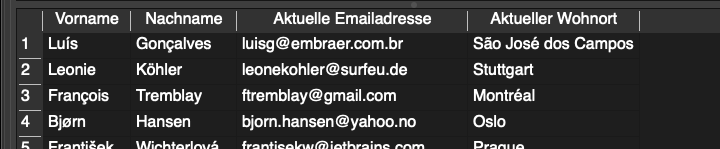
\includegraphics[width=10.41667in,height=\textheight]{img-SELECT5.png}

\hypertarget{order-by}{%
\section{ORDER BY}\label{order-by}}

Um unsere Ergebnisse nun auch zu soriteren, können wir den Befehl \textbf{ORDER BY} verwenden, die entsprechende Variable wählen und zwischen \textbf{ASC} für ascending (aufsteigend) und \textbf{DESC} für descending (absteigend) wählen. Verzichten wir auf die Angabe von \textbf{ASC} und \textbf{DESC}, wird immer \textbf{ASC} ausgewählt. Zur besseren Lesbarkeit empfiehlt es sich dennoch die Angabe zu definieren.

\begin{verbatim}
SELECT
  FirstName AS Vorname,
  LastName AS Nachname,
  Email AS 'Aktuelle Emailadresse',
  City AS [Aktueller Wohnort]
FROM
  customers
 ORDER BY
    FirstName ASC;
\end{verbatim}

\hypertarget{limit}{%
\section{LIMIT}\label{limit}}

Möchten wir die Ausgabe nun auch auf eine bestimmte Anzahl von Ergebnissen beschränken, können wir dies mit dem Befehl \textbf{LIMIT} tun:

\begin{verbatim}
SELECT
  FirstName AS Vorname,
  LastName AS Nachname,
  Email AS 'Aktuelle Emailadresse',
  City AS [Aktueller Wohnort]
FROM
  customers
 ORDER BY
    FirstName ASC
LIMIT 3;
\end{verbatim}

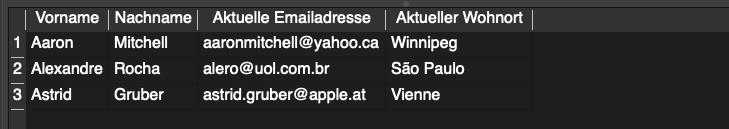
\includegraphics[width=10.41667in,height=\textheight]{img-SELECT6.png}

\hypertarget{where}{%
\section{WHERE}\label{where}}

Um Daten genauer filtern zu können und bestimmte Informationen ausfindig zu machen, können wir den Befehl \textbf{WHERE} nutzen. Dabei stößt man auf verschiedene Operatoren, die unsere Auswahl genauer bestimmen.

Zu diesen Operatoren zählen:

Vergleiche:\\
\textbf{= gleich}\\
\textbf{\textgreater{} größer als}\\
\textbf{\textless{} kleiner als}\\
\textbf{\textgreater= größer oder gleich}\\
\textbf{\textless= kleiner oder gleich}\\
\textbf{\textless\textgreater{} ungleich}

Logische Operatoren:\\
\textbf{BETWEEN}\\
\textbf{IN}\\
\textbf{LIKE}\\
\textbf{AND}\\
\textbf{OR}

Möchten wir nun zum Beispiel wissen, welche Rechnungen aus unserer \textbf{invoices} Tabelle einen \textbf{Gesamtbetrag von 1.98\$ (Total = 1.98)} aufweisen, wann die Bestellungen getätigt worden sind (InvoiceDate) und mit welcher Stadt (BillingCity) und Rechnungsadresse (BillingAddress) können wir folgenden Befehl ausführen:

\begin{verbatim}
SELECT
    InvoiceDate AS Bestelldatum,
    BillingAddress AS Rechnungsadresse,
    BillingCity AS Stadt,
    Total AS Betrag
FROM
    invoices
WHERE
    Total = 1.98
ORDER BY
    InvoiceDate;
\end{verbatim}

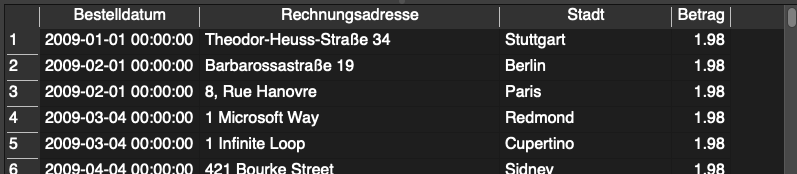
\includegraphics[width=10.41667in,height=\textheight]{img-WHERE1.png}

Ebenso können wir mit dem \textbf{BETWEEN} Operator herausfinden, welche Rechnungen einen Gesamtbetrag zwischen 1.98 und 5.00 aufweisen:

\begin{verbatim}
SELECT
    InvoiceDate AS Bestelldatum,
    BillingAddress AS Rechnungsadresse,
    BillingCity AS Stadt,
    Total AS Betrag
FROM
    invoices
WHERE
    Total BETWEEN 1.98 AND 5.00
ORDER BY
    InvoiceDate;
\end{verbatim}

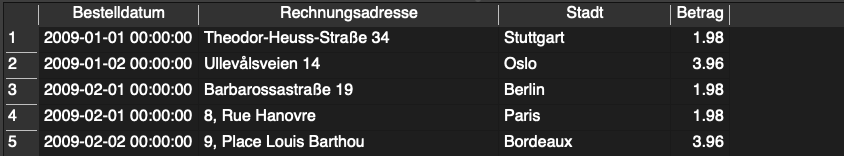
\includegraphics[width=10.41667in,height=\textheight]{img-WHERE2.png}

Um nach \textbf{Text-Daten} zu filtern, müssen wir den entsprechenden Text lediglich mit Anführungszeichen umschließen. So lassen sich zum Beispiel wie folgt alle Bestellungen aus Stuttgart abrufen:

\begin{verbatim}
SELECT
  InvoiceDate AS Bestelldatum,
  BillingAddress AS Rechnungsadresse,
  BillingCity AS Stadt,
  Total AS Betrag
FROM
  invoices
WHERE
  BillingCity = 'Stuttgart'
ORDER BY
  InvoiceDate;
\end{verbatim}

Dabei können wir ganz gleich ob es sich um Zahlenwerte oder Text handelt auch mehrere Kriterien verwenden. Möchten wir z.B. alle Rechnungen aus Stuttgart mit einem Betrag von mehr al 5\$, können wir dies durch \textbf{AND} hinzufügen:

\begin{verbatim}
SELECT
  InvoiceDate AS Bestelldatum,
  BillingAddress AS Rechnungsadresse,
  BillingCity AS Stadt,
  Total AS Betrag
FROM
  invoices
WHERE
  BillingCity = 'Stuttgart' AND Total > 5
ORDER BY
  InvoiceDate;
\end{verbatim}

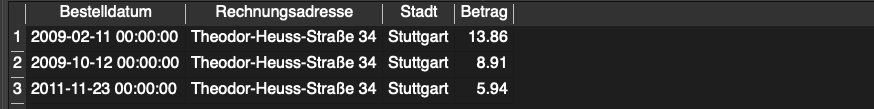
\includegraphics[width=10.41667in,height=\textheight]{img-WHERE3.png}

Durch den Operator \textbf{IN} können wir zudem festlegen, dass mehrere Ausprägungen einer Variable in Betracht gezogen werden sollen. So lassen sich wie folgt alle Rechnungen aus Stuttgart oder Berlin abfragen. Wir erhalten praktisch alle Einträge, bei denen der Wert der Variable BillingCity \textbf{in} unserer Liste vorkommt.

\begin{verbatim}
SELECT
  InvoiceDate AS Bestelldatum,
  BillingAddress AS Rechnungsadresse,
  BillingCity AS Stadt,
  Total AS Betrag
FROM
  invoices
WHERE
  BillingCity IN ('Stuttgart','Berlin')
ORDER BY
  InvoiceDate;
\end{verbatim}

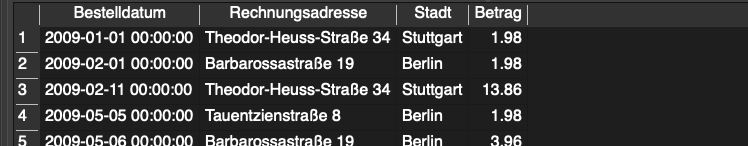
\includegraphics[width=10.41667in,height=\textheight]{img-WHERE4.png}

Wenn wir nach Ergebnissen suchen, die ein Kriterium nur teilweise erfüllen sollen, zum Beispiel alle Rechnungen von Städten, die mit ``B'' anfangen, können wir den Operator \textbf{LIKE} verwenden. Dabei ist durch ein \textbf{\%}-Zeichen zu definieren, ob die Buchstaben vor, hinter oder sowohl vor als auch hinter dem gewünschten Inhalt beliebige sind:

Durch \textbf{BillingCity LIKE `B\%'} erhalten wir alle Städte die mit B beginnen. (Brüssel, etc.)\\
Durch \textbf{BillingCity LIKE `\%T'} erhalten wir alle Städte die auf T enden. (Frankfurt, etc.)\\
Durch \textbf{BillingCity LIKE `\%k\%'} erhalten wir alle Städte die ein K beinhalten. (Stockholm, etc.)\\
Durch \textbf{BillingCity LIKE `O\%O'} erhalten wir alle Städte die mit O beginnen und enden. (Oslo, etc.)

\begin{verbatim}
SELECT
  InvoiceDate AS Bestelldatum,
  BillingAddress AS Rechnungsadresse,
  BillingCity AS Stadt,
  Total AS Betrag
FROM
  invoices
WHERE
  BillingCity LIKE '%K%'
ORDER BY
  InvoiceDate;
\end{verbatim}

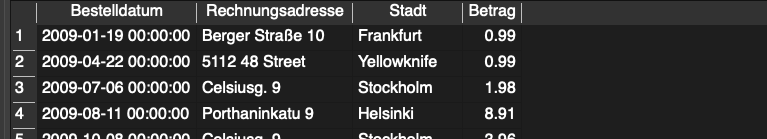
\includegraphics[width=10.41667in,height=\textheight]{img-WHERE8.png}

Nützlich wird dies vor allem in Situationen, in denen wir vielleicht nicht wissen wie genau die \textbf{Eingaben der Daten} erfolgt sind oder wir nach kurzen Inhalten in \textbf{langen Texten} filtern möchten. Suchen wir beispielsweise alle Rechnungen mit der Adresse \emph{``Berger Straße''} und wissen dabei nicht, ob das Wort \emph{Straße} in der Eingabe ausgeschrieben oder gekürzt wurden und um welche Hausnummer es sich handelt, können wir mit der folgenden Abfrage alle Einträge erhalten, in denen das Wort \emph{Berger} in der Rechnungsadresse vorgekommen ist:

\begin{verbatim}
SELECT
  InvoiceDate AS Bestelldatum,
  BillingAddress AS Rechnungsadresse,
  BillingCity AS Stadt,
  Total AS Betrag
FROM
  invoices
WHERE
  BillingAddress LIKE '%Berger%'
ORDER BY
  InvoiceDate;
\end{verbatim}

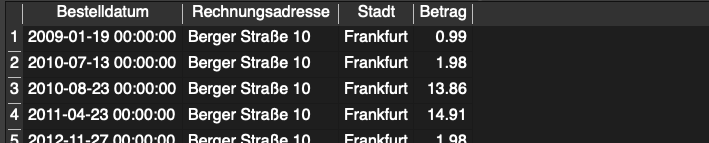
\includegraphics[width=10.41667in,height=\textheight]{img-WHERE5.png}

\hypertarget{nutzung-mehrerer-operatoren}{%
\section{Nutzung mehrerer Operatoren}\label{nutzung-mehrerer-operatoren}}

In der Realität werden diese Filter meist komplexer und verwenden mehrere Operatoren wie \textbf{AND} und \textbf{OR} zugleich. Dabei gilt es bestimmte Reihenfolgen und Regeln zu beachten, um nicht das falsche Ergebnis zu erhalten. Ohne die Verwendung von Klammern werden die Bedingungen auf beiden Seiten des \textbf{AND} automatisch zusammengefasst. Dies entspricht jedoch nicht immer unserem Vorhaben.

Möchten wir beispielsweise eine Liste aller Rechnungen mit einem \textbf{Betrag über 1.50\$} aus Städten die entweder \textbf{mit D oder P beginnen}, könnten wir die Bedingung \emph{Total \textgreater{} 1.50} über \textbf{AND} mit *BillingCity Like `p\%' OR BillingCity Like `d\%' verbinden. Ohne Klammern erhalten wir jedoch das folgende Ergebnis:

\begin{verbatim}
SELECT
  InvoiceDate AS Bestelldatum,
  BillingAddress AS Rechnungsadresse,
  BillingCity AS Stadt,
  Total AS Betrag
FROM
  invoices
WHERE
  Total > 1.50 AND BillingCity LIKE 'p%' OR BillingCity LIKE 'd%'
ORDER BY
  Total;
\end{verbatim}

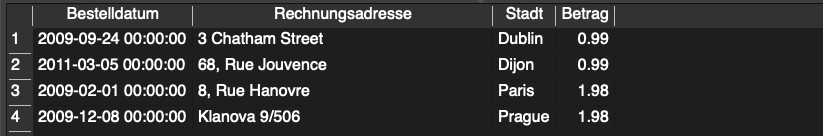
\includegraphics[width=10.41667in,height=\textheight]{img-WHERE6.png}

Wie wir an den ersten beiden Einträgen mit Betrag unter 1.50\$ sehen können, hat SQL unseren Befehl anders verstanden, als wir es uns gewünscht haben. Die beiden Kriterien vor dem \textbf{OR} wurden zusammengefasst, während alles nach dem \textbf{OR} einzeln und damit ohne Rücksicht auf den Betrag betrachtet wurde.
Wir haben also alle Einträge erhalten, die entweder der Bedingung ``\textbf{größer als 1.50\$ und aus Stadt mit p am Anfang}'' oder der Bedingung ``\textbf{Stadt mit d am Anfang}'' entsprechen.

Um das korrekte Ergebnis zu erhalten, müssen wir Klammern so setzen, dass alle Bedingungen korrekt interpretiert werden, also so, dass zunächst alle Rechnungen mit den gewünschten Beträgen gesucht und erst anschließend die weiteren Bedingungen angewendet werden.

\begin{verbatim}
SELECT
  InvoiceDate AS Bestelldatum,
  BillingAddress AS Rechnungsadresse,
  BillingCity AS Stadt,
  Total AS Betrag
FROM
  invoices
WHERE
  Total > 1.50 AND (BillingCity LIKE 'p%' OR BillingCity LIKE 'd%')
ORDER BY
  Total;
\end{verbatim}

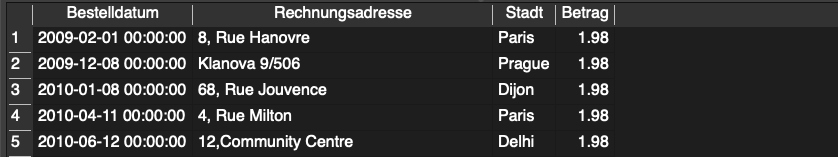
\includegraphics[width=10.41667in,height=\textheight]{img-WHERE7.png}

\hypertarget{mehrere-tabellen-verbinden}{%
\chapter{Mehrere Tabellen verbinden}\label{mehrere-tabellen-verbinden}}

Einer der wichtigsten Aspekte beim Nutzen von SQL ist die Fähigkeit Daten aus mehreren Tabellen zu erhalten. Wie wir in unserem \textbf{Datenbank-Schema} und dem Reiter \textbf{Datenbankstruktur} bereits festgestellt haben, befinden sich 13 Tabellen in unserer Datenbank, die wir über die \textbf{PRIMARY} und \textbf{FOREIGN KEYS} verknüpfen können. Der übergreifende Befehl dafür wird \textbf{JOIN} genannt und lässt sich auf beliebig viele Tabellen anwenden. Dabei unterscheidet man zwischen sogenannten \textbf{INNER} und \textbf{OUTER} \textbf{JOINS}, die wir uns in den folgenden Abschnitten genauer ansehen.

\hypertarget{inner-joins}{%
\section{Inner Joins}\label{inner-joins}}

Wie wir in unserem Datenbank-Schema feststellen konnten, besteht unsere Tabelle aus den Variablen \textbf{AlbumId}, \textbf{Title} und \textbf{ArtistId}. Möchten wir nun zu dem Albumtiteln auch Namen der Interpreten sehen, ist dies ohne die \textbf{artists} Tabelle nicht möglich. Da die Variable \textbf{ArtistId} in der \textbf{albums} Tabelle jedoch als \textbf{FOREIGN KEY} mit dem \textbf{PRIMARY KEY} \textbf{ArtistId} in der \textbf{artists} Tabelle übereinstimmt, können wir sie mit der folgenden Abfrage verbinden:

Wir verbinden die beiden Tabellen \textbf{albums} und \textbf{artists} bei allen Einträgen, bei denen die ArtistId in der Albums-Tabelle der ArtistId in der Artists-Tabelle entspricht.

\begin{verbatim}
SELECT
    *
FROM
    albums
INNER JOIN
    artists
ON
    albums.ArtistId = artists.ArtistId;
\end{verbatim}

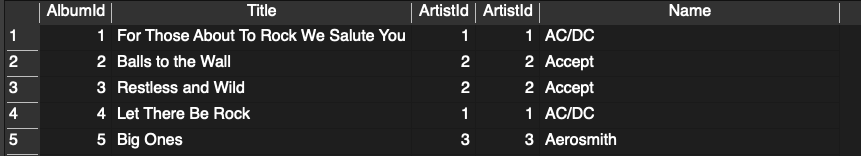
\includegraphics[width=10.41667in,height=\textheight]{img-JOIN1.png}

Dabei können wir den Code einfacher und übersichtlicher darstellen, indem wir den beiden Tabellen innerhalb der Abfrage ein \textbf{Alias} geben. So müssen wir die Tabellennamen nach ihrer ersten Benennung im Befehl nicht erneut ausschreiben:

\begin{verbatim}
SELECT
    *
FROM
    albums AS a
INNER JOIN
    artists AS n
ON
    a.ArtistId = n.ArtistId;
\end{verbatim}

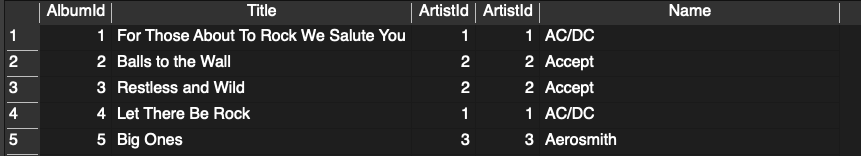
\includegraphics[width=10.41667in,height=\textheight]{img-JOIN1.png}

Wenn wir nun die Auswahl der Variablen eingrenzen, können wir dies ebenfalls mit dem Alias machen, selbst wenn dieser erst in den darauf folgenden Zeilen definiert wird:

\begin{verbatim}
SELECT
    a.Title,
    n.Name
FROM
    albums AS a
INNER JOIN
    artists AS n
ON
    a.ArtistId = n.ArtistId;
\end{verbatim}

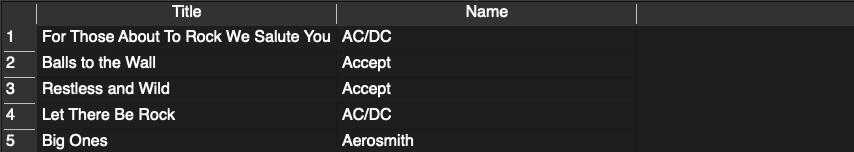
\includegraphics[width=10.41667in,height=\textheight]{img-JOIN2.png}

Zu beachten ist, dass \textbf{INNER JOINS} ausschließlich übereinstimmende Einträge wiedergeben. In unserem Beispiel passt es logischerweise, dass alle Alben jemandem zugeordnet werden können. Gibt es jedoch für einen Eintrag keine Übereinstimmung, wird dieser Eintrag bei einem \textbf{INNER JOIN} fallen gelassen. Durch unsere Abfrage erhielten wir alle Alben und die zum Album gehörenden Artists, da jedoch nicht von allen Artists ein Album in unserem Store ist, wurden einige bei dieser Abfrage ausgeschlossen - wie wir gleich sehen werden.

\hypertarget{outer-joins}{%
\section{Outer Joins}\label{outer-joins}}

\textbf{Outer Joins} geben \textbf{eine Tabelle vollständig} wieder und fügen die übereinstimmende Einträge einer anderen Tabelle der ersten hinzu. Man unterscheidet dabei zwischen sogenannten \textbf{LEFT OUTER JOINS} und \textbf{RIGHT OUTER JOINS}. Bei \textbf{LEFT OUTER JOINS} werden sozusagen allen Einträgen der ``linken Tabelle'' die passenden Einträge der ``rechten Tabelle'' hinzugefügt werden und alle Einträge ohne Übereinstimmung für die Variablen der rechten Tabelle Null-Werte erhalten.

Für \textbf{RIGHT OUTER JOINS} gilt dies auch, nur in umgekehrter Reihenfolge. Diese werden in SQLite nicht unterstützt, lassen sich aber logischerweise durch einen \textbf{LEFT OUTER JOIN} durch Tauschen der Tabellen replizieren.

Nehmen wir erneut das Beispiel mit den Alben und Artists. Möchten wir unsere \textbf{artists} Tabelle um Albuminformationen erweitern, auch wenn nicht alle Artists ein Album in unserem Store aufweisen, können wir den \textbf{LEFT OUTER JOIN} nutzen. Dabei nehmen wir die artists Tabelle auf die linke und die albums Tabelle auf die rechte Seite.

\begin{verbatim}
SELECT
    n.Name AS 'Artist-Name',
    a.Title AS 'Album-Titel'
FROM
    artists AS n
LEFT OUTER JOIN
    albums AS a
ON
    n.ArtistId = a.ArtistId;
\end{verbatim}

Scrollen wir jetzt ein wenig durch die Ergebnisse, sehen wir zum einen, dass wir für Künstler mit mehreren Alben auch mehrere Einträge haben, gleichzeitig jedoch immernoch alle Künstler ohne Album vorhanden sind. Überall, \textbf{wo keine Übereinstimmung mit der albums Tabelle gefunden worden ist, wurden Null-Werte hinzugefügt}:

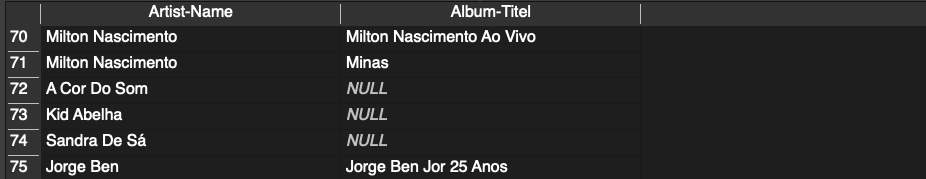
\includegraphics[width=10.41667in,height=\textheight]{img-JOIN3.png}

\hypertarget{nutzung-mehrerer-joins}{%
\section{Nutzung mehrerer Joins}\label{nutzung-mehrerer-joins}}

Bei Betrachtung unseres Datenbank-Schemas zeigt sich, dass sich noch mehr als nur zwei Tabellen miteinander verknüpfen lassen. Möchten wir beispielsweise wissen, welche Songs in einer Playlist vorkommen und wie Song und Playlist jeweils heißen, müssen wir die Tabellen \textbf{playlists}, \textbf{playlist\_track} und \textbf{tracks} verbinden.

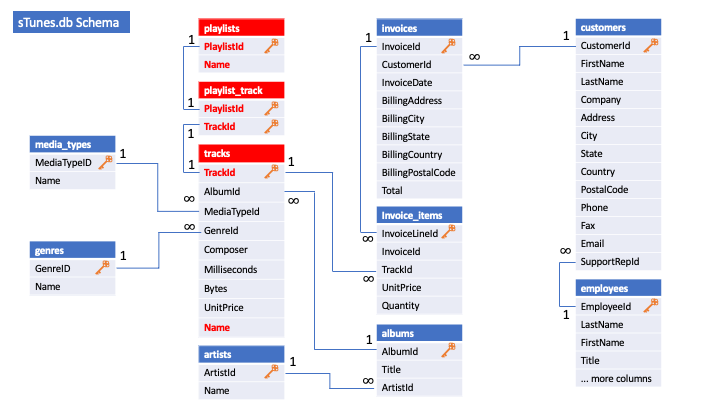
\includegraphics[width=11.45833in,height=\textheight]{img-sTunes-Schema3.png}

Durch einen \textbf{INNER JOIN} zwischen der \textbf{PlaylistId} in der Tabelle \textbf{playlists} und der \textbf{PlaylistID} in der Tabelle \textbf{playlist\_track} können wir zunächst alle Track-IDs, die in den jeweiligen Playlists vorkommen ausfindig machen. Anschließend können wir diese \textbf{TrackID} aus der Tabelle \textbf{playlist\_track} für einen weiteren \textbf{INNER JOIN} nutzen, um über die \textbf{TrackId} in der Tabelle \textbf{tracks} an die Variable \textbf{Name} des Tracks heranzukommen. Wir können also auf einen Join den nächsten folgen lassen:

\begin{verbatim}
SELECT
    p.name AS Playlistname,
    p.PlaylistId,
    t.TrackId,
    t.name AS Songname,
    t.Composer
FROM
    playlists AS p
INNER JOIN
    playlist_track AS pt
ON
    p.PlaylistId = pt.PlaylistId
INNER JOIN
    tracks AS t
ON 
    pt.TrackId = t.TrackId
ORDER BY
    p.PlaylistId DESC;
\end{verbatim}

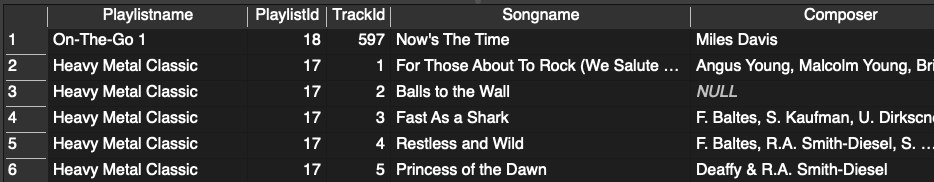
\includegraphics[width=10.41667in,height=\textheight]{img-JOIN4.png}

\hypertarget{erweiterte-sql-abfragen}{%
\chapter{Erweiterte SQL-Abfragen}\label{erweiterte-sql-abfragen}}

In der Praxis wird man uns natürlich nicht nur damit beauftragen, bestimmte Einträge aus der Datenbank zu ziehen, sondern diese auch auszuwerten, gesondert aufzubereiten und für das Management relevante Schlussfolgerungen anzustellen. Als abschließenden Ausblick, schauen wir uns nun ein paar erweiterte SQL-Abfragen in Kurzform an.

\hypertarget{aggregatfunktionen}{%
\section{Aggregatfunktionen}\label{aggregatfunktionen}}

Ein wichtiges Element in der Arbeit mit Datenbanken sind Aggregatfunktion, also Funktionen mit denen wir Daten zusammenfassen oder mathematische Berechnungen anstellen können. Die folgenden fünf grundlegenden Aggregatfunktionen sind dabei nur ein kleiner Teil der in SQL verwendbaren Funktionen:

\begin{itemize}
\tightlist
\item
  \textbf{AVG()}\\
\item
  \textbf{COUNT()}\\
\item
  \textbf{MAX()}\\
\item
  \textbf{MIN()}\\
\item
  \textbf{SUM()}
\end{itemize}

Angewendet werden diese Funktionen wie folgt:

\begin{verbatim}
SELECT
    SUM(Total) AS Summe,
    AVG(Total) AS Durchschnittsbetrag,
    MAX(Total) AS 'Höchster Betrag',
    MIN(Total) AS 'Geringster Betrag',
    COUNT(*) AS 'Anzahl der Belege'
FROM
    invoices;
\end{verbatim}

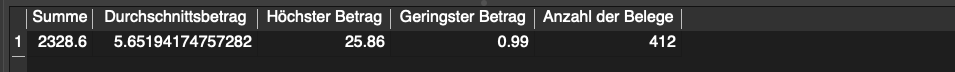
\includegraphics[width=10.41667in,height=\textheight]{img-FUNC1.png}

\textbf{COUNT()} beachtet dabei nur Werte die nicht Null sind. In unserem Beispiel haben wir jedoch mit dem * in der Klammer alle Null und Error-Werte mitgezählt.

Wie wir anhand des Durchschnittsbetrags sehen können, hat SQL das Ergebnis nicht gerundet. Zum Runden können wir die Funktion \textbf{ROUND(X,Y)} verwenden, wobei X für den Wert der gerundet werden soll und Y für Anzahl der Nachkommastellen steht.

\begin{verbatim}
SELECT
    SUM(Total) AS Summe,
    AVG(Total) AS Durchschnittsbetrag,
    ROUND(AVG(Total), 2) AS 'Gerundeter Durchschnittsbetrag',
    MAX(Total) AS 'Höchster Betrag',
    MIN(Total) AS 'Geringster Betrag',
    COUNT(*) AS 'Anzahl der Belege'
FROM
    invoices;
\end{verbatim}

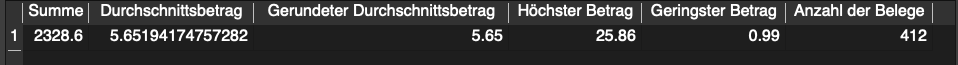
\includegraphics[width=10.41667in,height=\textheight]{img-FUNC2.png}

\hypertarget{group-by}{%
\section{GROUP BY}\label{group-by}}

In den meisten Fällen werden wir beispielsweise jedoch nicht einfach nach dem Durchschnittswert der gesamten Tabelle, sondern nach dem Durchschnitt in bestimmten Kategorien oder Gruppen gefragt.

Um Werte für bestimmte Gruppen berechnen zu können, lässt sich der Befehl \textbf{GROUP BY} verwenden. So können wir wie im folgenden Beispiel die Durchschnittsbeträge der Rechnungen je nach Stadt darstellen:

\begin{verbatim}
SELECT
    BillingCity AS Standort,
    AVG(Total) AS 'Durchschnittlicher Rechnungsbetrag'
FROM
    invoices
GROUP BY
    BillingCity;
\end{verbatim}

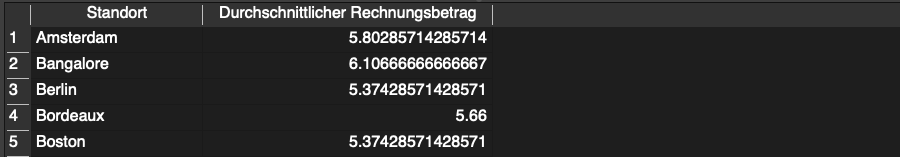
\includegraphics[width=10.41667in,height=\textheight]{img-FUNC3.png}

Möchten wir dabei wie in den vorherigen Kapiteln nach bestimmten Eigenschaften filtern, können wir auch hier den Befehl \textbf{WHERE} einsetzen. So können wir uns wie folgt die Durchschnittsbeträge für alle Städte mit F als Anfangsbuchstaben ausgeben lassen:

\begin{verbatim}
SELECT
    BillingCity AS Standort,
    AVG(Total) AS 'Durchschnittlicher Rechnungsbetrag'
FROM
    invoices
WHERE
    BillingCity LIKE 'F%'
GROUP BY
    BillingCity;
\end{verbatim}

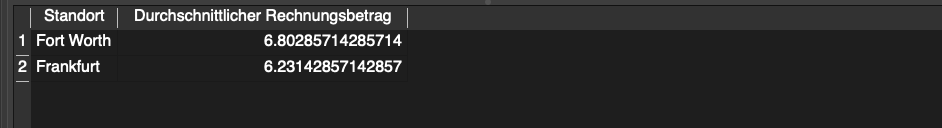
\includegraphics[width=10.41667in,height=\textheight]{img-FUNC4.png}

Sollten wir jedoch nach dem Ergebnis unserer Aggregatfunktion filtern wollen, können wir \textbf{WHERE} nicht verwenden. Möchten wir z.B. nur Städte sehen, dessen Durchschnittsbetrag größer als 6 ist und definieren dies wie folgt durch \textbf{WHERE}, erhalten wir eine Fehlermeldung:

\begin{verbatim}
SELECT
    BillingCity AS Standort,
    AVG(Total) AS 'Durchschnittlicher Rechnungsbetrag'
FROM
    invoices
WHERE
    AVG(Total) > 6
GROUP BY
    BillingCity;
\end{verbatim}

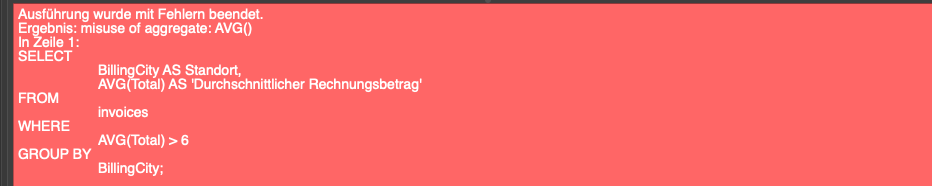
\includegraphics[width=10.41667in,height=\textheight]{img-FUNC5.png}

Um nach dem Ergebnis der Aggregatfunktion filtern zu können, müssen wir den Befehl \textbf{HAVING} nach dem \textbf{GROUP BY} Befehl einsetzen:

\begin{verbatim}
SELECT
    BillingCity AS Standort,
    AVG(Total) AS 'Durchschnittlicher Rechnungsbetrag'
FROM
    invoices
GROUP BY
    BillingCity
HAVING
    AVG(Total) > 6;
\end{verbatim}

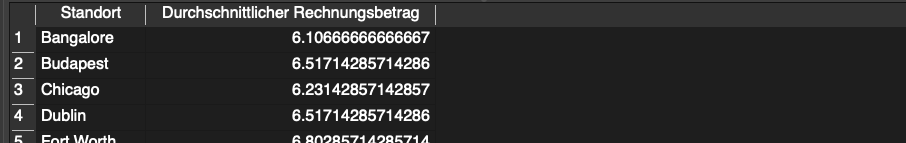
\includegraphics[width=10.41667in,height=\textheight]{img-FUNC6.png}

Wir können festhalten, dass \textbf{WHERE} als Filter für direkte Daten aus unseren Tabellen und \textbf{HAVING} als Filter für aggregierte Daten genutzt werden kann. Der Befehl \textbf{HAVING} führt ohne \textbf{GROUP BY} zu einem Error.

Selbstverständlich können wir beide Befehle auch zusammen verwenden. Beispielsweise um uns alle Städte mit Anfangsbuchstabe F (Werte aus der Tabelle) mit einem Durchschnittsbetrag über 6 (Werte die wir neu berechnen) ausgeben zu lassen. Hierbei ist die Reihenfolge der Befehle \textbf{FROM}, \textbf{WHERE}, \textbf{GROUP BY} und \textbf{HAVING} entscheidend:

\begin{verbatim}
SELECT
    BillingCity AS Standort,
    AVG(Total) AS 'Durchschnittlicher Rechnungsbetrag'
FROM
    invoices
WHERE
    BillingCity LIKE 'B%'
GROUP BY
    BillingCity
HAVING
    AVG(Total) > 6;
\end{verbatim}

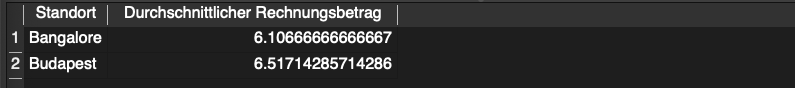
\includegraphics[width=10.41667in,height=\textheight]{img-FUNC7.png}

\hypertarget{case}{%
\section{CASE}\label{case}}

In manchen Szenarien möchten wir die Fälle in unserer Tabelle aufgrund bestimmter Werte zu neuen Gruppen zuteilen. Beispielsweise um zwischen kleinen, mittleren und großen Bestellungen zu unterscheiden. Durch den Befehl \textbf{CASE} können wir diese Zuteilung vornehmen. Der Befehl wird in unserer Auswal der Variablen im Befehl \textbf{SELECT} platziert und definiert die Zuteilung zu einer bestimmten Gruppe je nach Wert einer anderen Variable.

\begin{verbatim}
SELECT
    InvoiceDate AS Bestelldatum,
    BillingAddress AS Rechnungsadresse,
    Total AS Rechnungsbetrag,
    CASE
    WHEN Total < 2.00 THEN 'Kleine Bestellung'
    WHEN Total BETWEEN 2.00 AND 7.00 THEN 'Mittlere Bestellung'
    ELSE 'Große Bestellung'
    END AS Bestellungsumfang
FROM
    invoices;
\end{verbatim}

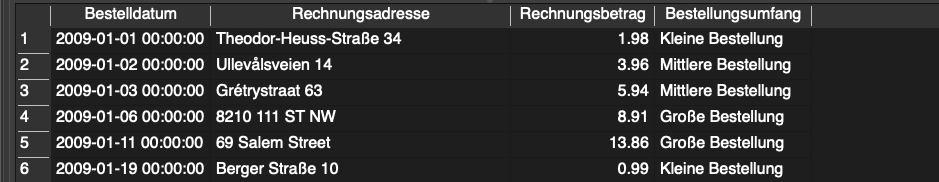
\includegraphics[width=10.41667in,height=\textheight]{img-FUNC8.png}

So wählen wir wie im folgenden Codeblock zunächst die Variablen unserer Tabelle, die wir uns anzeigen lassen möchten, und platzieren dann unseren Befehl \textbf{CASE}. Ohne die darauf folgenden Zeilen mit einem Komma zu trennen, wie es bei den Variablen der Fall ist, definieren wir dann mit dem Wort \textbf{WHEN}, unter welchen Umständen \emph{(Total \textless{} 2.00)} der jeweilige Fall zu einer neuen Kategorie \emph{(Kleine Bestellung)} hinzugefügt werden soll. Das Wort \textbf{ELSE} teilt dann alle Fälle, die den vorherigen \textbf{WHEN} Bedingungen nicht entsprechen einer weiteren Kategorie zu. Der CASE Befehl wird dann durch \textbf{END AS} mit dem Namen unserer neuen Spalte beendet.

Möchten wir anschließend nurnoch die großen Bestellungen betrachten, können wir wieder durch \textbf{WHERE} filtern:

\begin{verbatim}
SELECT
    InvoiceDate AS Bestelldatum,
    BillingAddress AS Rechnungsadresse,
    Total AS Rechnungsbetrag,
    CASE
    WHEN Total < 2.00 THEN 'Kleine Bestellung'
    WHEN Total BETWEEN 2.00 AND 7.00 THEN 'Mittlere Bestellung'
    ELSE 'Große Bestellung'
    END AS Bestellungsumfang
FROM
    invoices
WHERE
    Bestellungsumfang = 'Große Bestellung';
\end{verbatim}

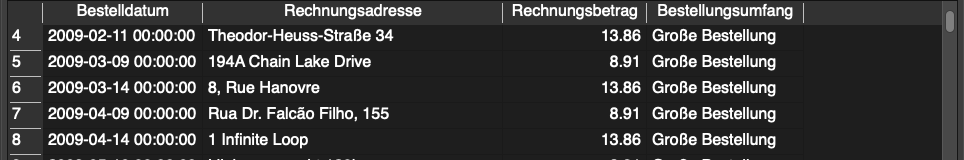
\includegraphics[width=10.41667in,height=\textheight]{img-FUNC9.png}

\hypertarget{erstellung-von-datenbanken}{%
\chapter{Erstellung von Datenbanken}\label{erstellung-von-datenbanken}}

Die letzten Grundlagen, mit denen man sich beschäftigen sollte, bevor man sich mit komplexeren Abfragen und Funktionen auseinandersetzt, umfassen das Erstellen von Datenbanken und Tabellen.

Die Datenbankerstellung im DB Browser for SQLite ist etwas anders, als bei der Nutzung gängiger Datenbanksysteme, weshalb das folgende Beispiel im DB Browser nicht anwendbar ist.

In gängigen Datenbanksystemen lässt sich eine neue Datenbank einfach über den Befehl \textbf{CREATE DATABASE} in Kombination mit dem Namen der neuen Datenbank erstellen:

\begin{verbatim}
CREATE DATABASE datenbankname;
\end{verbatim}

Anschließend lässt sich eine neue Tabelle in der Datenbank über den Befehl \textbf{CREATE TABLE} erstellen. Dabei müssen für jede Spalte, die wir erstellen wollen, der Spaltenname und der Datentyp der jeweiligen Spalte definiert werden:

\begin{verbatim}
CREATE TABLE Playlistkuratoren (
    KuratorId INT NOT NULL,
    Personalnummer INT,
  Vorname NVARCHAR(40),
    Nachname NVARCHAR(40),
  Geburtsdatum DATE,
  PlaylistAnzahl NUMERIC(4),
    PRIMARY KEY (KuratorId),
    FOREIGN KEY (Personalnummer) REFERENCES employees(EmployeeId)
)
\end{verbatim}

In diesem Beispiel erstellen wir eine neue Tabelle, in der wir Daten über die Kuratoren von Playlisten sammeln.

In der ersten Spalte soll sich unsere \emph{KuratorId} befinden, diese ist vom Typ \textbf{INT} - also Integer, eine ganze Zahlen. Durch \textbf{NOT NULL} legen wir fest, dass dieses Feld für keinen Eintrag in der Tabelle leer sein darf - denn mit der ID wollen wir den jeweiligen Eintrag immer identifizieren können.

Da einige Kuratoren eventuell direkt bei uns angestellt sind, möchten wir zudem eine Spalte für mögliche Personalnummern mit dem Datentyp \textbf{INT} anlegen.

Für Vor- und Nachname nehmen wir den Datentyp \textbf{NVARCHAR}. Es kann also ein beliebig langer Text eingegeben werden, der jedoch durch den Zusatz \textbf{(40)} auf maximal 40 Zeichen begrenzt ist.

Für das Geburtsdatum wählen wir den Datentyp \textbf{DATE}.

Durch den \textbf{PRIMARY KEY} legen wir nun fest, welche Variable als Primary Key dienen soll und damit jeder Wert der Variable nur einmal vorkommen kann. Zusätzlich legen wir fest, dass unsere Variable \emph{Personalnummer} als \textbf{FOREIGN KEY} für die Variable \emph{employeeId} in der Tabelle \emph{employees} dient.

Nun ist unsere neue Tabelle erstellt und wir müssen diese nurnoch mit Einträgen befüllen. Dies geschieht mit den Befehl \textbf{INSERT INTO}, bei dem we´ir die entsprechende Playlist und die zu befüllenden Spalten auswählen und anschließend über \textbf{VALUES} die Daten eingeben:

\begin{verbatim}
INSERT INTO Playlistkuratoren (KuratorId, Personalnummer, Vorname, Nachname, Geburtsdatum, PlaylistAnzahl)
VALUES (2,1,'Andrew', 'Adams', '1962-02-18',3);
\end{verbatim}

Möchten wir jetzt beispielsweise wissen, wie die Email-Adressen von Mitarbeitern sind, die unsere Playlisten zusammenstellen, können wir den folgenden \textbf{INNER JOIN} benutzen:

\begin{verbatim}
SELECT
    p.KuratorId,
    p.Personalnummer,
    p.PlaylistAnzahl,
    e.FirstName,
    e.LastName,
    e.Email
FROM
    employees AS e
INNER JOIN
    Playlistkuratoren AS p
ON
    p.Personalnummer = e.EmployeeId;
\end{verbatim}

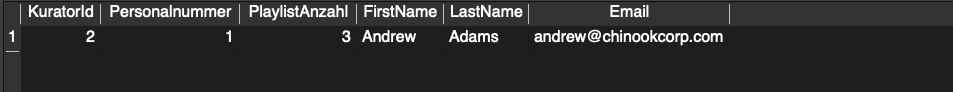
\includegraphics[width=10.41667in,height=\textheight]{img-CREATE1.png}

Logischerweise sehen wir, dass es nur den einen, neu hinzugefügten Mitarbeiter gibt, der als Playlistkurator tätig ist.

  \bibliography{book.bib,packages.bib}

\end{document}
